\end{multicols}

\begin{figure}[H]
    \centering
    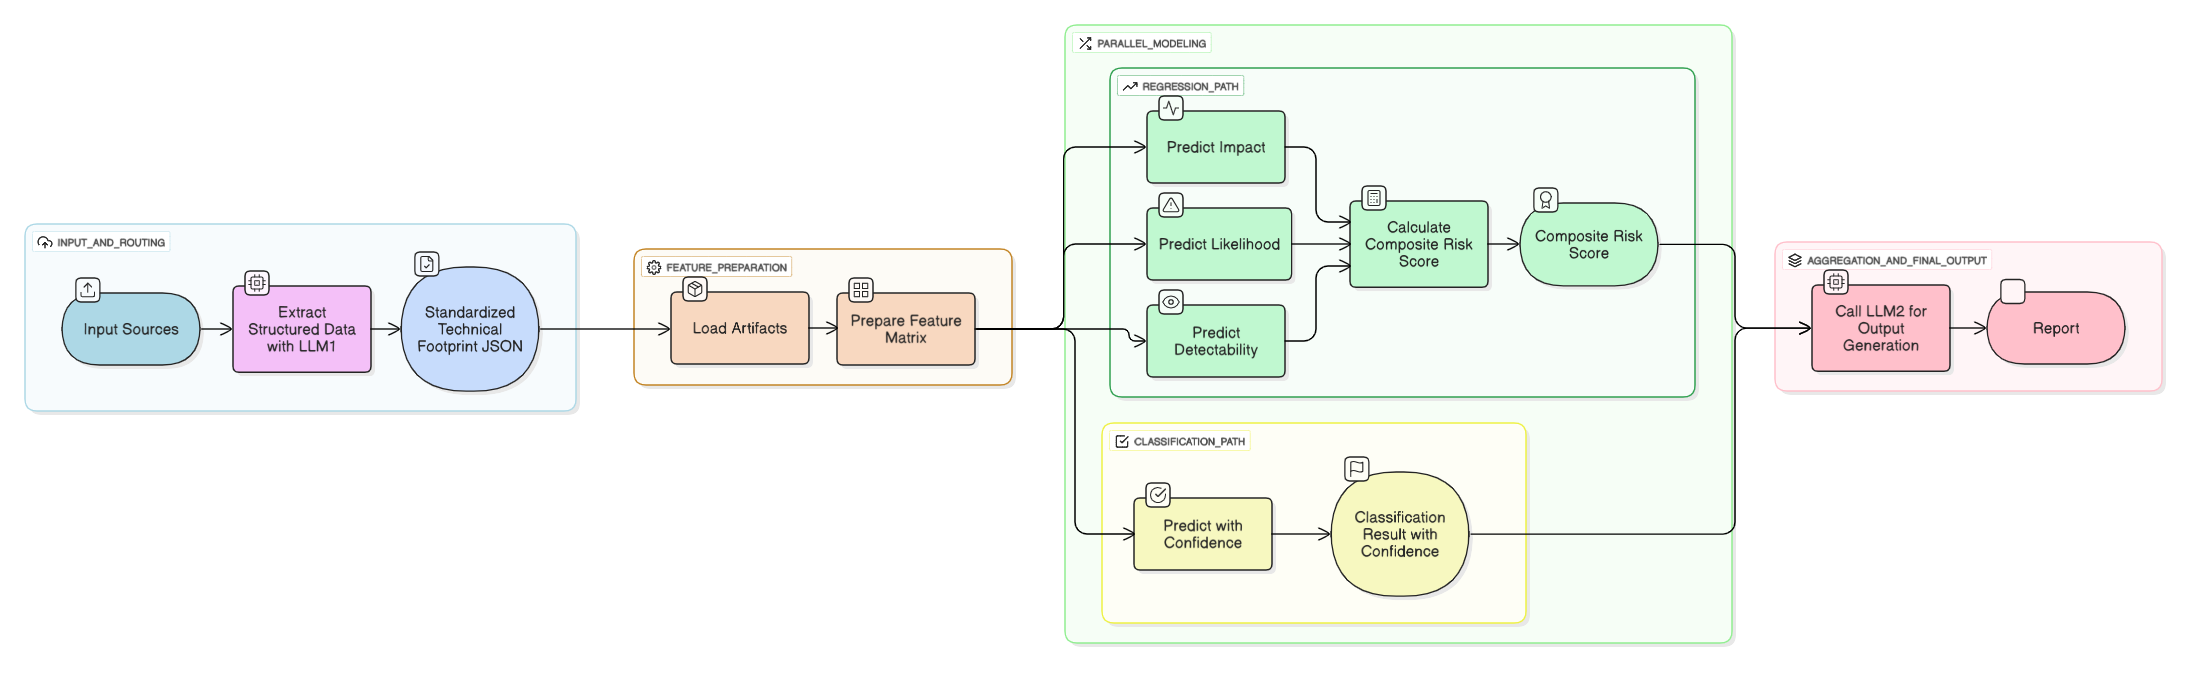
\includegraphics[width=\textwidth]{../figure/methodology/pipeline.jpg}
    \caption{The architecture of our model for blockchain security framework.}
    \label{fig:pipeline_architecture}
\end{figure}

\begin{multicols}{2}

\subsection{Automated Pipeline: LLM-Assisted Extraction and ML Prediction}
\label{sec:ml_pipeline}

We complement the checklist-first assessment with an implemented automated pipeline that transforms enterprise documentation into predictions and an executive-ready report. The pipeline follows three stages: LLM extraction, ML prediction, and LLM reporting. Models were trained and evaluated on the labeled incident dataset, and a worked example is provided below.

\subsubsection{Stage 1: LLM Extraction to Technical Footprint}
An LLM ingests enterprise documents (whitepapers, internal runbooks, API docs) and produces a structured technical footprint. The schema below is used as model features and for auditability:
\begin{itemize}
    \item \textbf{chain} (string, mandatory): Operational blockchain instance (e.g., Avalanche C-Chain, Ethereum)
    \item \textbf{platform\_type} (string, mandatory): Technology family (e.g., EVM, Substrate, Cosmos SDK)
    \item \textbf{consensus\_mechanism} (string): PoW, PoS, BFT, etc.
    \item \textbf{audit\_status} (string): Audit status (e.g., Not Audited, Audited by Tier-1 Firm)
    \item \textbf{key\_management} (string): Privileged key management (e.g., EOA, 3-of-5 Multisig, HSM)
    \item \textbf{oracle\_dependency} (string): Price oracle design (e.g., Spot Price from DEX, TWAP, Chainlink Feed)
    \item \textbf{economic\_exploit\_vectors} (string list): Economic primitives (e.g., Flash Loan, Liquidity Manipulation)
    \item \textbf{code\_level\_defenses} (string list): Relevant code patterns/libraries (e.g., Reentrancy Guard, SafeMath)
    \item \textbf{vulnerability\_source} (string, training-only): Root cause label used for training (e.g., Smart Contract Bug, Economic Design Flaw). Not surfaced in end-user reports.
\end{itemize}

\textit{Note:} The technical footprint is stored with provenance pointers to the source snippets used by the LLM.

\subsubsection{Stage 2: ML Prediction (XGBoost)}

\begin{figure}[H]
    \centering
    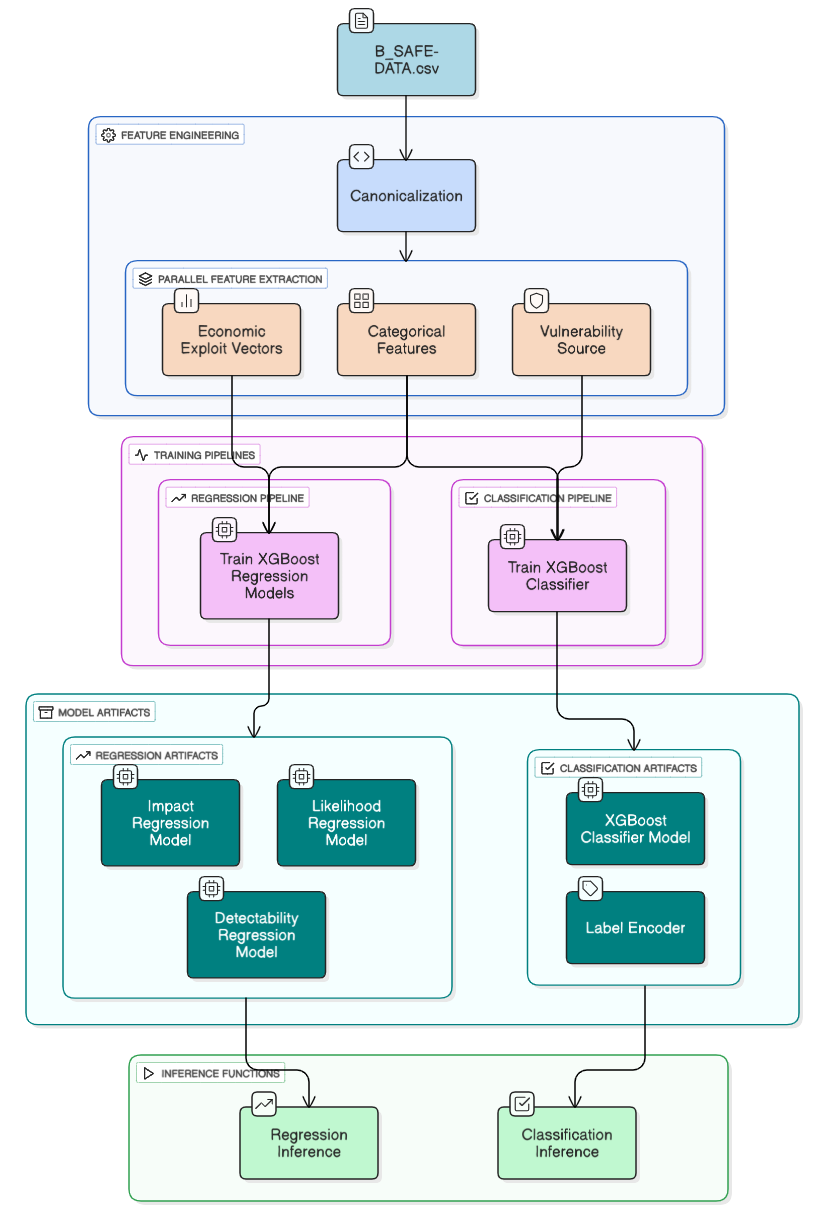
\includegraphics[width=0.4\textwidth]{../figure/methodology/ml.png}
    \caption{The architecture of machine learning models.}
    \label{fig:machine_learning}
\end{figure}

We train two XGBoost models using the labeled incident dataset and the extracted technical footprints, and we report held-out validation performance:
\begin{itemize}
    \item \textbf{Risk Dimension Regressor}: Multi-target regression predicting Likelihood (L), Impact (I), Detectability (D), each on 1--5 scales. Targets derive from manual grading performed during data curation.
    \item \textbf{Risk Category Classifier}: Multi-class classifier predicting the risk category (e.g., SC-1 Reentrancy, PRO-2 Oracle Manipulation, AUX-1 Private Key Compromise), with calibrated confidence.
\end{itemize}
Categorical features are one-hot encoded; list features are multi-hot encoded; numeric features remain numeric. We stratify by category for training/validation to prevent leakage.

\subsubsection{Stage 3: LLM Reporting}
Predictions are combined with checklist outcomes to generate a concise executive report: priority ranking (Critical/High/Medium/Low), primary/secondary predicted vulnerabilities with confidence, and prioritized recommendations tied to actionable controls. The end-to-end pipeline output is demonstrated in the worked example below.

\paragraph{Worked Example: ``Project Equinox''}
\textbf{Input excerpt} (enterprise whitepaper): Avalanche C-Chain; decentralized lending; PoS; oracle: spot price from DEX (Trader Joe); flash loans supported; admin via 3-of-5 multisig; audited by CertiK; reentrancy guards present.

\textbf{Extracted technical footprint} (abridged):
\begin{itemize}
    \item chain: Avalanche C-Chain; platform\_type: EVM; consensus\_mechanism: PoS
    \item oracle\_dependency: Spot Price from DEX; economic\_exploit\_vectors: [Flash Loan]
    \item key\_management: 3-of-5 Multisig; audit\_status: Audited by Tier-1 Firm
    \item code\_level\_defenses: [Reentrancy Guard]
    \item vulnerability\_source (training-only): Economic Design Flaw
\end{itemize}

\textbf{Model outputs} (illustrative): Critical Priority ranking; \textit{Primary} category: PRO-2 Oracle Manipulation (high confidence); \textit{Secondary} category: AUX-2 Governance Attack (moderate confidence). L, I, and D predicted by the regressor support the priority ranking calculation.

\textbf{Recommendations}: Replace spot DEX price with manipulation-resistant oracles (e.g., TWAP or Chainlink feeds), and harden key management SOP for multisig participants (HSM-backed storage, break-glass procedures, periodic access reviews).

\subsubsection{Positioning}
The automated pipeline accelerates assessments and surfaces statistically grounded risks. It is designed to complement---not replace---the checklist and human review. Final decisions remain human-in-the-loop.


